En este sector, se busca resolver el problema de CMF a partir de una Heurística de Búsqueda Tabú (Tabu search\footnote{Glover, F. "Tabu Search — Part I", ORSA Journal on Computing 1989}). Dicha heurística consiste en una estrategia para resolver problemas combinatorios, aplicable tanto en grafos como en otras estructuras utilizadas para resolver problemas de lógica. Este método utiliza el mismo procedimiento que Búsqueda Local\footnote{Ver sección anterior.} para acercarse progresivamente a una mejor solución dentro de un entorno. Dado que en ciertos casos la solución no puede ser mejorada, la técnica de Búsqueda Tabú permite empeorarla parcialmente para proseguir la búsqueda de una mejor. A su vez, esta heurística concede una estructura llamada $lista\ tabu$ con distintas utilidades. Principalmente, sirve para guardar movimientos de modo a no repetirlos y/o guardar características o soluciones, entre otras. A continuación, se encuentra explicitado el pseudocódigo\footnote{http://www.dc.uba.ar/materias/aed3/2013/2c/laboratorio/heuristicas.pdf} de la heurística de Búsqueda Tabú:

\begin{algorithm}[H]
\SetAlgoLined
s$_{0}$ $\leftarrow$ solucion inicial \\
s$^{*}$ $\leftarrow$ s$_{0}$ \\
T $\leftarrow$ lista tabu inicial \\
\While{ no se alcance el criterio de terminacion}{
N $\leftarrow$ vecinos de s no tabu o mejores que s$^{*}$ \\
s $\leftarrow$ mejor solucion en N. \\
\If{ s es mejor que s$^{*}$}
 {s$^{*}$ $\leftarrow$ s} 
Actualizar la lista tabu T }
\end{algorithm}

\subsection{Explicación del algoritmo realizado}

 El algoritmo realizado parte de un valor entero positivo ingresado como parámetro, $desviacion\_permitida$, y de una solución provista por la Heurística de Búsqueda Local. A partir de esta última, el algoritmo busca, paulatinamente, una mejor solución siguiendo las siguientes opciones:
\begin{itemize}
 \item Agregando un nodo: Dada la solución actual (una clique), procede a $agregar$ un nodo que la mejore, es decir, que aumente su frontera.
 \item Quitando un nodo: Dada la solución actual (una clique), procede a $quitar$ un nodo que la mejore, es decir, que aumente su frontera.
\end{itemize}
A diferencia de la Búsqueda Local, se buscan nuevas soluciones que no necesariamente mejoren la solución obtenida hasta el momento pero que sí lo hagan a largo plazo. Sin embargo, dentro de las formas de empeorar la solucion, se toma aquella que empeora lo menos posible. A su vez, a medida que agregamos o quitamos un nodo lo vamos poniendo en la lista tabu. Esto lo hace sin olvidar que siempre que pueda subir lo va a hacer, entonces, si descendiendo se encuentra con que puede volver a ascender, lo va a hacer hasta volver a estar en un máximo local.\newline

\begin{figure}[H] %[h] Aqui [b] para button [t] para top
\begin{center}
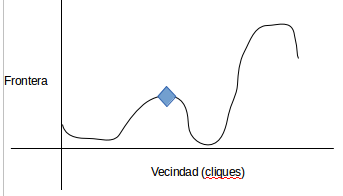
\includegraphics[width=250pt]{../imgs/1_tabu.png}
\caption{Solucion con Busqueda Local}
\end{center}
\end{figure}


\begin{figure}[H] %[h] Aqui [b] para button [t] para top
\begin{center}
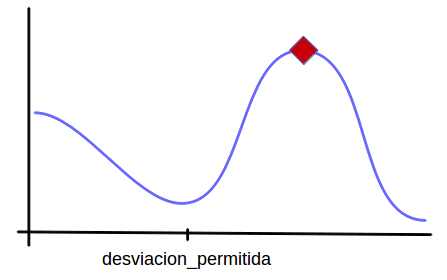
\includegraphics[width=250pt]{../imgs/2_tabu.png}
\caption{Solucion con Busqueda Tabu}
\end{center}
\end{figure}

Al finalizar, el algoritmo retorna la mejor solución hallada. \newline

\textbf{Descripcion de la lista tabu} \newline

 A medida que se van agregando o quitando nodos que no mejoran la solucion estos nodos se van marcando como tabu. De esta forma se le asigna una prioridad a cada nodo que depende de cuando fue agregado. A su vez, sea cual sea la prioridad del ultimo agregado, no se puede utilizar en la iteracion siguiente, esto es para evitar ciclar soluciones. Esto lo logramos haciendo que en el peor de los casos solo se puedan usar los nodos tabus que tienen prioridad menor a la mitad de la prioridad maxima. \newline

\textbf{Criterio de terminacion} \newline

 La terminacion de este algoritmo va a estar dada por dos factores, por un lado, la cantidad de iteraciones en que la solucion puede mejorar, y por otro, por la variable $desviacion\_permitida$ ingresada como parametro. El primero es seguro que es acotado ya que el maximo absoluto esta dado por la solucion exacta del problema, entonces, puede haber muchos maximos locales pero ninguno va a superar el maximo absoluto (esto es trivial). Por otro lado, la variable $desviacion\_permitida$ va disminuyendo cada vez que modifico la solucion actual sin mejorarla, es decir, que permitimos avanzar de manera "no creciente" una cantidad $desviacion\_permitida$ de veces. \newline


\begin{algorithm}[H]
    \SetAlgoLined
    \caption{TabuSearch}
    \KwIn{\textbf{Conj(nodos)} $solución\_inicial$, \textbf{Grafo} $g$, \textbf{Entero} $desviacion\_permitida$}
    \KwOut{\textbf{Conj(nodos)} $solución\_final$}

	\textbf{Conj(nodos)} sol$_{0}$,sol$_{1}$ \\ 
	\textbf{Conj(nodos)} $solución\_actual$ $\leftarrow$ LocalSearch($solución\_inicial$, $g$)	\\	
	\textbf{Conj(nodos)} $solución\_final$ $\leftarrow$ $solución\_actual$	\\	
	\textbf{Lista Tabu} $\leftarrow$ $\{\}$\\
	\textbf{Boolean} $Mejore\ la\ frontera$ $\leftarrow$ true

	\While{ $Mejore\ la\ frontera$ $\vee$ 0 $<$ $desviacion\_permitida$}{

	 	sol$_{0}$ $\leftarrow$ Dame Mejor solucion agregando nodo No Tabu ($solución\_inicial$,$solución\_final$) \\
		sol$_{1}$ $\leftarrow$ Dame Mejor solucion quitando nodo No Tabu ($solución\_inicial$,$solución\_final$) \\
		\If{ frontera(sol$_{0}$) $<$ frontera(sol$_{1}$)}
			{sol$_{0}$ $\leftarrow$ sol$_{1}$}
		\eIf{ frontera($solución\_actual$) $<$ frontera(sol$_{1}$)}
			{$solución\_actual$ $\leftarrow$ sol$_{0}$ \\
			$Mejore\ la\ frontera$ $\leftarrow$ true
			}
			{$Mejore\ la\ frontera$ $\leftarrow$ false \\
			 Poner Tabu Nodo utilizado en sol$_{0}$ \\
			 $desviacion\_permitida$ - 1}
		$solución\_actual$ $\leftarrow$ sol$_{0}$ \\
		\If{ frontera($solución\_final$) $<$ frontera($solución\_actual$) } 
		{$solución\_final$ $\leftarrow$ $solución\_actual$}			
	}

    	\textbf{devolver} $solución\_final$ \\

\end{algorithm}

\begin{algorithm}[H]
    \SetAlgoLined
    \caption{Dame Mejor solucion agregando nodo No Tabu}

	$solución\_final$ $\leftarrow$ $solución\_inicial$ con un nodo mas cualquiera \\
	\ForAll{$u \in Candidatos\_clique($solución\_inicial$)$}{
	 		\If{$u$ $\notin Nodos(solución\_inicial)$}{
				\eIf{$\neg$ es tabu($u$)}{
		 			\If{frontera($solución\_final$) $<$ frontera( $solución\_inicial$ con $u$) }{
						$solución\_final$ $\leftarrow$ $solución\_inicial$ con $u$}
				}{
					\If{ Es Tabu aceptable ($u$) $\land$ frontera($solución\_final$) $<$ frontera( $solución\_inicial$ con $u$)}
					{$solución\_final$ $\leftarrow$ $solución\_inicial$ con $u$}
				
				}
			}
	}

\end{algorithm}

\begin{algorithm}[H]
    \SetAlgoLined
    \caption{Dame Mejor solucion quitando nodo No Tabu}

	$solución\_final$ $\leftarrow$ $solución\_inicial$ sin un nodo cualquiera \\
	\ForAll{$u \in$ Nodos($solución$\_$inicial$)}{
		\eIf{$\neg$ es tabu($u$)}{
	 		\If{frontera($solución\_final$) $<$ frontera( $solución\_inicial$ sin $u$)}{
	 			$solución\_final$ $\leftarrow$ $solución\_inicial$ sin $u$}
		}{
				\If{Es Tabu aceptable ($u$) $\land$ frontera($solución\_final$) $<$ frontera($solución\_inicial$ con $u$)}
					{$solución\_final$ $\leftarrow$ $solución\_inicial$ con $u$}
		}
	}

\end{algorithm}

Donde:
\begin{itemize}
 \item $desviacion$\_$permitida$ Dice la cantidad de veces que se agrega o quita un nodo por iteracion (empeorando la solución parcial).
 \item frontera : Dice, dada una solución como parametro, el numero de nodos adyacentes a la frontera (es lo que pide maximizar el enunciado).
 \item Candidatos$\_$clique : Dice los nodos que pertenecen a la clique maxima de los nodos pasados como parametro.
 \item Nodos : Da los nodos pertenecientes a la solución pasada como parametro.
 \item Es Tabu aceptable : Un nodo perteneciente a la lista tabu es aceptable si su prioridad es menor a la mitad de la prioridad maxima.
\end{itemize}

\subsection{Complejidad Temporal}

 Para desarrollar la complejidad de este algoritmo comencemos estudiando las estructuras y las formas en las que guardamos los datos. \newline

 Cuando nos referimos a una "solución" en el código esta plasmado como una estructura ($solucionTabu$) que consiste en dos listas\footnote{http://www.cplusplus.com/reference/list/list/}, $adentro$ y $candidatos$, un vector\footnote{http://www.cplusplus.com/reference/vector/vector/} $esta$ y un entero $cantFrontera$:
\begin{itemize}
 \item $adentro$: Lista que indica los nodos que contiene mi solución actual.
 \item $candidato$: Lista de los nodos candidatos a formar una clique máxima (teniendo en cuenta los nodos de $adentro$). 
 \item $esta$: Vector booleano de nodos que están en mi solución.
 \item $cantFrontera$: Entero que indica la frontera de mi solución.\newline
\end{itemize}
 Como puede apreciarse $adentro$, $candidato$ y $esta$ están acotados por la cantidad de nodos. De esta manera, copiar una solución consiste en copiar dichas estructuras y eso es lineal en el tamaño, es decir, 3.$cant.nodos$ = O($cant.nodos$). 
 Gracias a $cantFrontera$ solicitar la frontera de una solución sea constante, ya que es solo retornar el elemento. A su vez, operaciones como agregar o quitar un nodo consisten en realizar los siguientes pasos: \newline
\begin{itemize}
 \item $Copiar\ una\ solucion$ actual a una nueva (como ya vimos es lineal en la cantidad de nodos)
 \item $Quitar\ o\ agregar\ un\ nodo$ de $esta$ y $adentro$. Ponerlo como ausente en $esta$ es constante (es solo acceder al nodo) y eliminarlo de la lista es lineal en la cantidad de elementos a eliminar\footnote{http://www.cplusplus.com/reference/list/list/erase/}, pero como solo eliminamos uno, es constante. Por otro lado, agregar un elemento en $esta$ es constante (por el mismo argumento anterior) y agregarlo a la lista también lo es\footnote{http://www.cplusplus.com/reference/list/list/push_back/}.
 \item $Calcular\ los\ candidatos$ donde borramos la lista anterior de candidatos\footnote{http://www.cplusplus.com/reference/list/list/clear/} (esto es lineal en la cant. de nodos en el peor caso) y luego se recorren todos los nodos, a su vez de todos los que estan en $adentro$ para ver adyacencias (esto tiene un costo de $(cant.nodos)$$^{2}$) mientras que se va insertando los que corresponden\footnote{http://www.cplusplus.com/reference/list/list/push_back/}.
 \item $Calcular\ la\ frontera$ consiste en recorrer los nodos de $adentro$ (lineal en cant. de nodos) y luego restarles la cantidad de nodos de la clique (que es $n*(n-1)$ con $n$=nodos de la clique)
\end{itemize}
 Siendo así que agregar o quitar un nodo tienen un costo de O($cant.nodos$) + O(1) + O(1) + O($cant.nodos$$^{2}$) + O($cant.nodos$) = O($cant.nodos$$^{2}$).\newline

 Por otro lado, la lista Tabu esta representada por un vector de $cant.nodos$ elementos donde en la i-esima posición esta el "valor tabu" del i-esimo nodo. Por lo tanto, poner como tabu a un nodo o ver su valor es equivalente a acceder\footnote{http://www.cplusplus.com/reference/vector/vector/operator[]/} a un elemento del arreglo que es constante.\newline

 Teniendo en cuenta todo lo anterior, empecemos viendo las complejidades de las funciones $Dame$ $Mejor$ $solucion$ $agregando$ $nodo$ $No$ $Tabu$ y $Dame$ $Mejor$ $solucion$ $agregando$ $nodo$ $No$ $Tabu$. Como se puede observar en los algoritmos ambas son son similares en cuanto a las operaciones realizadas, a diferencia que una agrega y la otra elimina nodos, pero como vimos antes, estas operaciones tienen similar complejidad. Por esta razón, procederemos a mostrar la complejidad de una y la otra es equivalente.\newline
 En primer lugar se copia una solución (O(cant.nodos)), luego para cada nodo candidato nos fijamos si pertenece a la solución (O(1)) y si no es el caso, entonces procede a fijarse si es tabu (O(1)) o si es "tabu aceptable" (O(1)), en cualquiera de los casos compara la solución final con la solución actual con un nodo agregado (comparar es constante al igual que ver la frontera y agregar un nodo es cuadrático en la cantidad de nodos) y por ultimo, de cumplirse las anteriores condiciones, copia el nodo actual con un nodo agregado a la mejor solución (copiar es lineal y agregar el nodo cuadrático en la cantidad de nodos). \newline
 Por estas razones la complejidad final de la función es O($cant.nodos$$^{2}$) + O($cant.nodos$) * (O(1)+O($cant.nodos$$^{2}$)) = O($cant.nodos$$^{3}$).\newline

 Solo queda ver la complejidad de la función principal "TabuSearch". Esta comienza realizando una búsqueda local\footnote{ver sección anterior} (O($cant.nodos$$^{2}$)) la cual es almacenada en una solución (guardar dicha solución cuesta cuadrático en la cantidad de nodos); seguido define la lista tabu en 0 todos los valores (lineal en cantidad de nodos). Continuando empieza un ciclo ($desviacion_permitida$ + $subida$ iteraciones, con $subida$ = cant. iteraciones en las que la frontera aumenta) y por cada iteración se ejecuta las funciones $Dame$ $Mejor$ $solucion$ $agregando$ $nodo$ $No$ $Tabu$ y $Dame$ $Mejor$ $solucion$ $agregando$ $nodo$ $No$ $Tabu$ (O($cant.nodos$$^{2}$)) seguido de comparaciones (constantes) y asignaciones con coste lineal. \newline
 De esta manera la complejidad final del algoritmo es O($cant.nodos$$^{4}$) + O($cant.nodos$$^{2}$) + O($cant.nodos$) * O($cant.nodos$$^{2}$) = O($cant.nodos$$^{4}$) , notando que $subida$ es a lo sumo $cant.nodos$ ya que en el peor caso puede ir de 0 a $cant.nodos$ (por eso la complejidad de ese ciclo queda lineal). 


\subsection{Instancias problemáticas}

 Aquí detallaremos instancias donde nuestra heuristica no encuentra soluciones cercanas a las optimas, o aun peor, se puede empeorar la solución cuanto uno quiera.

\begin{itemize}
 
  \item $La$ $solucion$ $inicial$ $va$ $a$ $condicionar$ $la$ $final$. Como la solución inicial se encuentra en un máximo local solo le queda a la búsqueda "descender" en busca de un "nuevo ascenso" (Con ascender o descender nos referimos a mejorar o empeorar la solución actual respectivamente). Dado que buscamos empeorar la solución actual lo menos posible, aquí se produce una intensificación. Veamos algunos ejemplos:

  \item $El$ $conjunto$ $de$ $cliques$ $sepadaras$ $afectan$ $la$ $solucion$. Cuando tenemos varias cliques máximas separadas, nosotros empezamos a explorar en una (que es donde la búsqueda local termino), si la solución optima se encuentra en otra clique a la que nuestra solución inicial no incide, el algoritmo difícilmente la halle. Por ejemplo:

\end{itemize}

Se puede observar como la mayoría de problemas encontrados se deben al proceso de intensificación, aunque en muchos casos puede ser muy favorable, en otros seria mejor aplicar técnicas de diversificación, como por ejemplo, variar la entrada por nodos de diferentes cliques máximas, colaborando mucho en la búsqueda de soluciones mas diversas.

\subsection{Experimentación}

 En esta sección buscamos encontrar un numero correcto para asignarle $desviacion_permitida$ de tal forma de amortiguar lo mas posible tiempo con resultados y por otro lado, probamos el algoritmo con diferentes instancias y así ver cuanto tardan .
